\chapter{Estimation Process}

\label{ch: Estim}

Parameter estimation problems can be interpreted as optimization problems, where one must find the optimal values of parameters in order to reduce the error between real system and model. During the years, many methods were developed to address this problem, but two approaches have been largely employed to obtain its solution. 

The first approach applies metaheuristics to obtain a sufficiently good solution. These methods are used in a variety of cases, ranging from biological to engineering problems, due to the fact that they are not developed for a specific type of problem. Metaheuristics employ a stochastic search to encounter (near-)optimal solutions within a given region. However, they often take a great amount of time to converge to a solution \cite{Blum2003}. Examples of metaheuristics are Ant Colony Optimization, Differential Evolution, Particle Swarm Optimization and Genetic Algorithm. Applications of this approach in electrical power system cases can be found in \cite{Todorovski2006} and \cite{Yoshida2000}.

The second approach applies analytical methods to find a global/local optimum solution. These methods use equations derived from the problem to locate an optimal solution. Thus, they are problem specific and must be adapted from one case to another. Analytical methods often converge in few iterations, reducing processing time, but are sensitive to initial conditions.

In this work is proposed to combine both approaches, reducing the effects of their disadvantages and improving overall convergence. Mean-Variance Mapping Optimization (MVMO) was the metaheuristic chosen for this problem, alongside Trajectory Sensitivity Method (TS) as analytical method. Both methods will be discussed in the following sections.

The flowchart depicted in Figure \ref{fig: flowchart} illustrates how the proposed method works. At first, a disturbance occurs, resulting in a dynamic response of the real system. The real system's outputs are compared to the model behaviour when the same disturbance is applied to it. The error $J(p)$ is evaluated and while it is greater than a given tolerance $t_{1}$, MVMO algorithm will search for a local solution. Afterwards, the error will eventually drop to a value lower than $t_{1}$, and TS will be used to refine the search to a optimal solution, with error level below $t_{2}$. The error will be evaluated through the Least-Squares Method, given by equation \ref{eq: J(p)}, where $y_{r}$ and $y$ stand for the real system and model outputs.

\begin{equation}
	J(p) = \frac{1}{2}\int\displaylimits_{0}^{T_{0}}(y_{r}(t) - y(t))^{T}(y_{r}(t) - y(t))dt
	\label{eq: J(p)}
\end{equation}

\begin{figure}
	\caption{Flowchart of estimation method}
	\begin{center}
		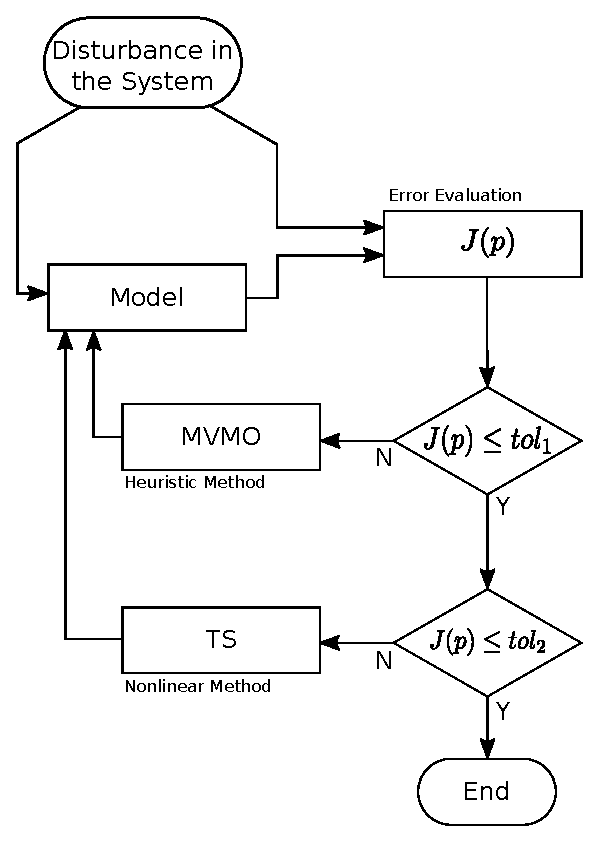
\includegraphics[scale=0.7]{Images/Flowchart.eps}
	\end{center}
	\label{fig: flowchart}
\end{figure}

\section{Mean-Variance Mapping Optimization}

Presented in \cite{Erlich2010}, this population-based metaheuristic shares characteristics with other evolutionary algorithms, but differ from them on how to induce mutations on the offspring in order to diversify the population. By considering statistical data of population during mutation process, MVMO introduces a memory factor to it, enhancing search mechanism. Due this factor, MVMO performs better than similar metaheuristics when population size is relatively small \cite{Nakawiro2011}.

Before the search process starts, a few settings must be done, such as population size, number of offspring, number of genes selected for mutation and selection method. Also, the search region is defined by setting the range within genes can vary. This constrains their values within a feasible region, preventing divergence. The search region is later normalized for all genes, aiding the process. Termination criteria is also set in this step. In this work, both number of generations and fitness will be used as stop criteria.





\section{Trajectory Sensitivity Method}